%%%%%%%%%%%%%%%%%%%%%%%%%%%%%%%%%%%%%%%%%%%%%%%%%%%%%%%%%%
% Reinforcement Learning Presentation                   %
% Authors: Abdelhakim Zetati & Lahcen Ezzara            %
% Date: Oct 2024                                        %
%%%%%%%%%%%%%%%%%%%%%%%%%%%%%%%%%%%%%%%%%%%%%%%%%%%%%%%%%%

\documentclass[serif, aspectratio=169]{beamer}
%\documentclass[serif]{beamer}  % for 4:3 ratio
\usepackage[T1]{fontenc} 
\usepackage{fourier} % see "http://faq.ktug.org/wiki/uploads/MathFonts.pdf" for other options
\usepackage{hyperref}
\usepackage{latexsym,amsmath,xcolor,multicol,booktabs,calligra}
\usepackage{graphicx,pstricks,listings,stackengine}
\usepackage{lipsum}

\author{Abdelhakim Zetati -- Lahcen Ezzara}
\title{Reinforcement Learning (RL)}
\subtitle{Tendances IT}
\institute{
   zetati.abdelhakim@ensam-casa.ma -- ezzara.lahcen@ensam-casa.ma \\
    Université Hassan II de Casablanca \\
    ENSAM Casablanca \\
}
\date{\small \today}
\usepackage{style}

% defs
\def\cmd#1{\texttt{\color{red}\footnotesize $\backslash$#1}}
\def\env#1{\texttt{\color{blue}\footnotesize #1}}
% set colors
\definecolor{hkustyellow}{RGB}{167, 131, 55}
\definecolor{hkustblue}{RGB}{0, 56, 116}
\definecolor{hkustred}{RGB}{209, 51, 59}


\lstset{
    basicstyle=\ttfamily\small,
    keywordstyle=\bfseries\color{deepblue},
    emphstyle=\ttfamily\color{deepred},    % Custom highlighting style
    stringstyle=\color{deepgreen},
    numbers=left,
    numberstyle=\small\color{halfgray},
    rulesepcolor=\color{red!20!green!20!blue!20},
    frame=shadowbox,
}

%- --- --- --- --- --- --- --- --- --- --- --- --- --- --- --- 
\begin{document}

\begin{frame}
    \titlepage
    \vspace*{-0.6cm}
    \begin{figure}[htpb]
        \begin{center}
            
\includegraphics[keepaspectratio, scale=0.15]{images/ensam-casa.png}
        \end{center}
    \end{figure}
\end{frame}

\begin{frame}    
\tableofcontents[sectionstyle=show,
subsectionstyle=show/shaded/hide,
subsubsectionstyle=show/shaded/hide]
\end{frame}

% Introduction au RL --- --- --- --- --- --- --- --- --- --- --- --- 

\section{Introduction au RL}

\begin{frame}{Comprendre l'Apprentissage par Renforcement}
	\frametitle<presentation>{Comprendre l'Apprentissage par Renforcement}
	\begin{block}{Reinforcement Learning (RL):}
		\begin{itemize}
			\item \textbf{L'apprentissage par renforcement (RL)} se distingue en apprenant à travers des interactions avec un environnement pour maximiser une fonction de récompense, sans étiquettes correctes prédéfinies, ce qui le rend utile pour la prise de décision dans des environnements complexes.
		\end{itemize}
	\end{block}
\end{frame}

% Interface Agent-Environnement --- --- --- --- --- --- --- --- --- --- --- ---

\section{Interface Agent-Environnement}

\begin{frame}{L'Interface Agent-Environnement d'un Système d'Apprentissage par Renforcement}
	\frametitle<presentation>{L'Interface Agent-Environnement d'un Système d'Apprentissage par Renforcement}
	
	L'état de l'agent est composé de ses variables, et il interagit avec l'environnement à travers des actions, recevant des récompenses qui guident ses transitions d'état. Le processus d'apprentissage implique de trouver un équilibre entre l'exploration (essayer de nouvelles actions) et l'exploitation (choisir des actions avec des récompenses connues) pour maximiser les récompenses cumulées au fil du temps. 
	
\end{frame}

\begin{frame}{L'Interface Agent-Environnement d'un Système d'Apprentissage par Renforcement}
	
	\begin{figure}[htpb]
		\centering
		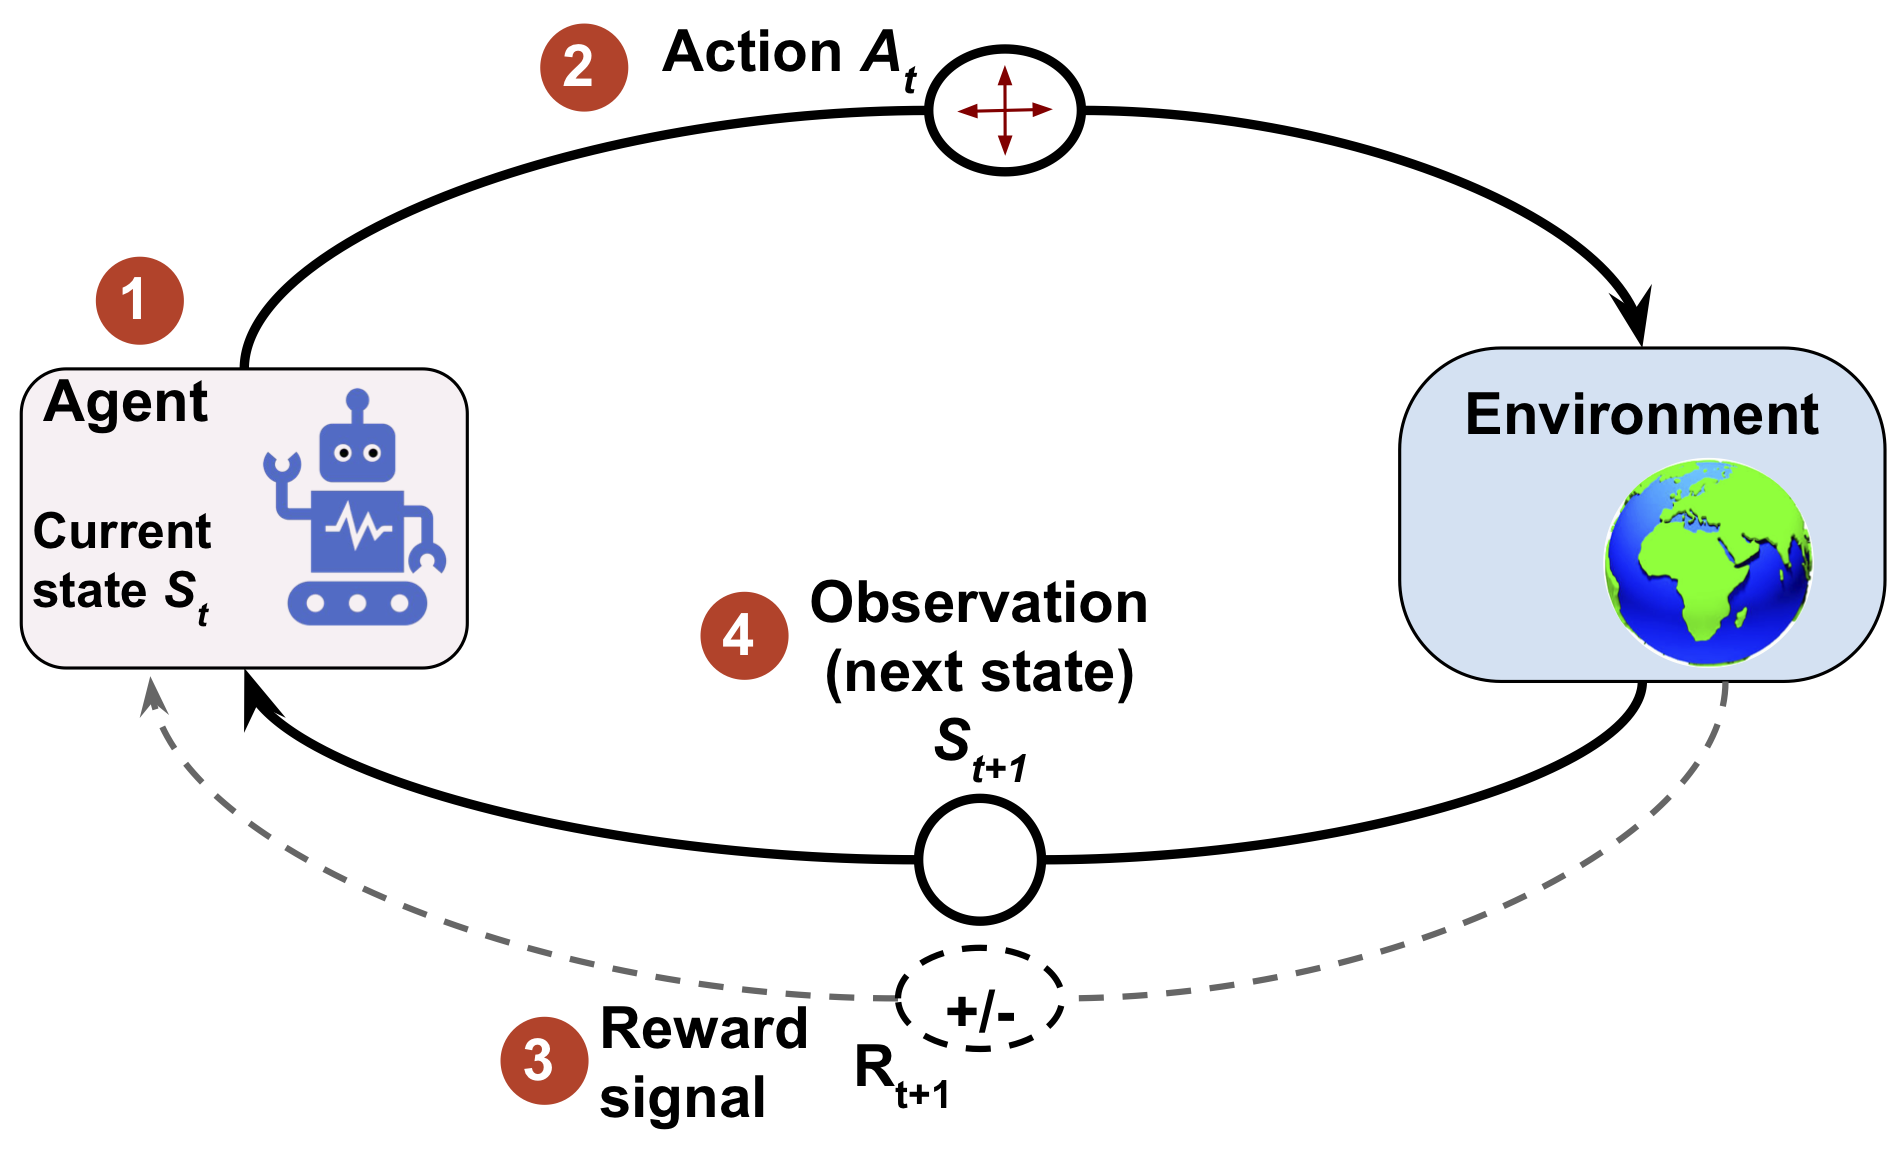
\includegraphics[keepaspectratio, scale=0.6]{images/interface-agent-environnement.png}
		\caption{L'Interface Agent-Environnement d'un Système d'Apprentissage par Renforcement}
		\label{fig:agent-environment}
	\end{figure}
	
\end{frame}


% Fondations Théoriques --- --- --- --- --- --- --- --- --- --- --- 
\section{Fondations Théoriques}

\begin{frame}{Les Processus de Décision de Markov}
	\frametitle<presentation>{Les Processus de Décision de Markov}
	
	En général, le type de problèmes que l'apprentissage par renforcement (RL) traite est généralement formulé comme des processus de décision de Markov (MDP). L'approche standard pour résoudre les problèmes MDP est d'utiliser la programmation dynamique, mais l'apprentissage par renforcement offre certains avantages clés par rapport à la programmation dynamique. 
	
\end{frame}

\begin{frame}{La Formulation Mathématique des Processus de Décision de Markov}
	\frametitle{La Formulation Mathématique des Processus de Décision de Markov}
	
	La distribution de probabilité pour \( S_{t+1} = s' \) et \( R_{t+1} = r \) peut être écrite comme une probabilité conditionnelle sur l'état précédent \( S_t \) et l'action prise \( A_t \) comme suit :
	
	\[
	p(s', r \mid s, a) \equiv P(S_{t+1} = s', R_{t+1} = r \mid S_t = s, A_t = a)
	\]
	
	\vspace{20pt}
	
	Deux approches principales pour traiter ce problème sont les méthodes Monte Carlo (MC) sans modèle et les méthodes de différence temporelle (TD). Le tableau suivant présente les deux principales catégories et les branches de chaque méthode :
	
\end{frame}

\begin{frame}{La Formulation Mathématique des Processus de Décision de Markov}
	\frametitle{La Formulation Mathématique des Processus de Décision de Markov}
	
	\begin{figure}[htpb]
		\centering
		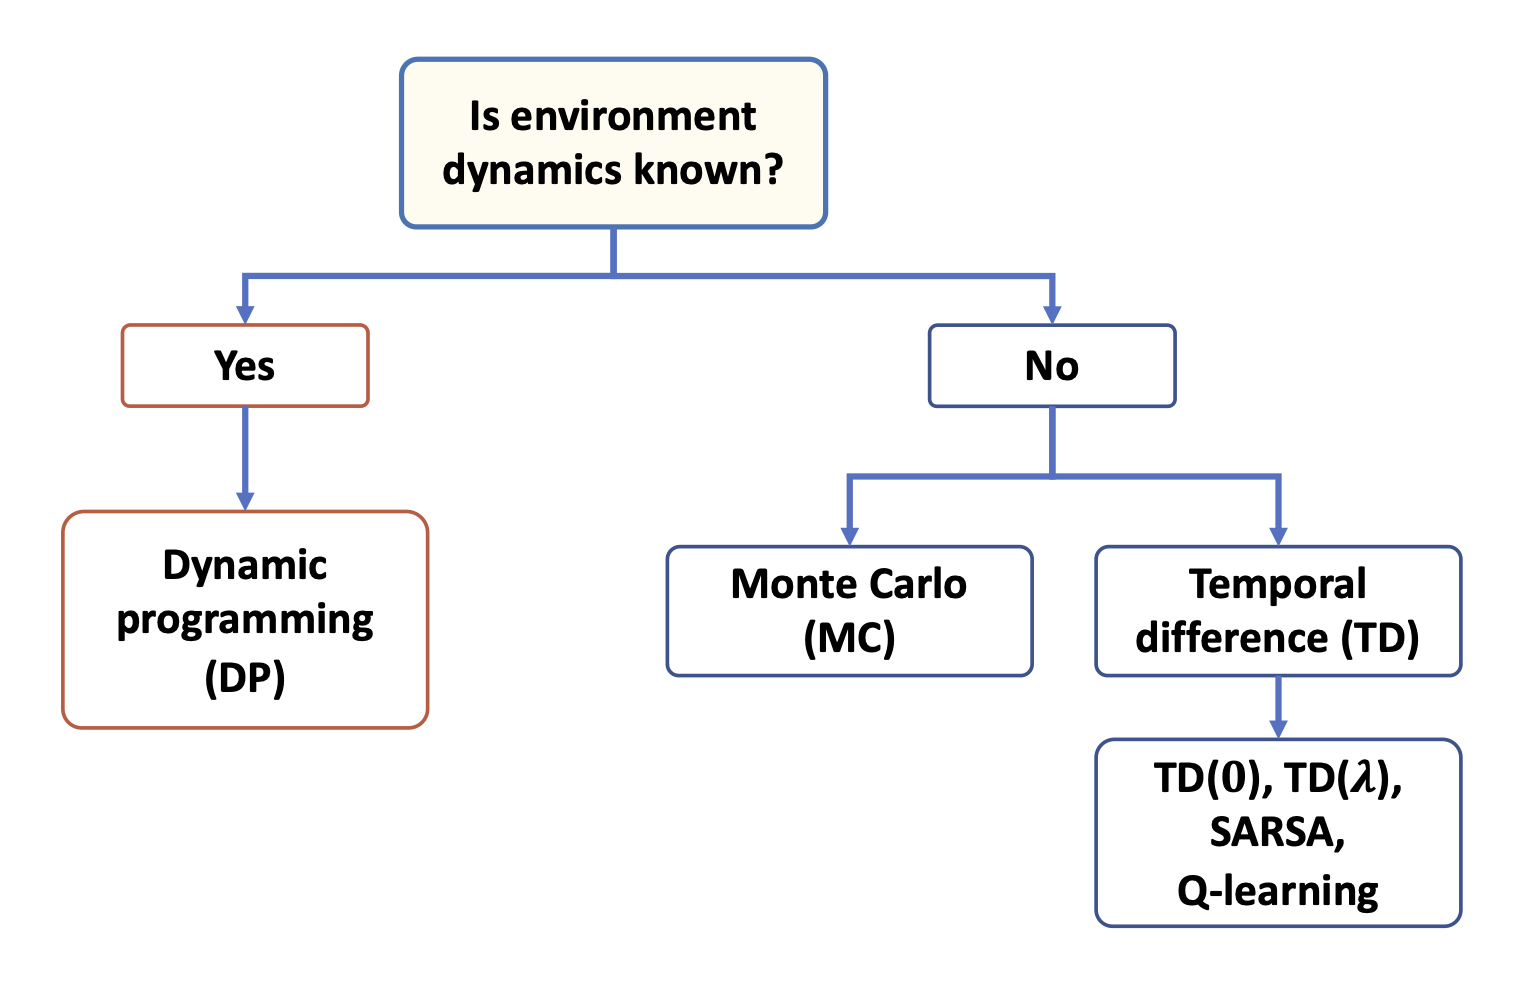
\includegraphics[keepaspectratio, scale=0.8]{images/markov.png}
	\end{figure}
	
\end{frame}


\begin{frame}{La Formulation Mathématique des Processus de Décision de Markov}
	\frametitle{La Formulation Mathématique des Processus de Décision de Markov}
		
		La dynamique de l'environnement peut être considérée comme déterministe si des actions particulières pour des états donnés sont toujours ou jamais prises, c'est-à-dire \(p(s', r \mid s, a) \in \{0,1\}\). Sinon, dans le cas plus général, l'environnement aurait un comportement stochastique.
		
\end{frame}


% Terminologie du RL --- --- --- --- --- --- --- --- --- --- --- 
\section{Terminologie du RL}

\begin{frame}{Lorem Ipsum Dolor Sit Amet}
	\frametitle{Lorem Ipsum Dolor Sit Amet}
	
	Lorem ipsum dolor sit amet, consectetur adipiscing elit. Vivamus dignissim mi et faucibus interdum. Etiam nisl sapien, auctor in hendrerit non, laoreet auctor dolor. Pellentesque vel ex id dui blandit porttitor ut vitae risus.
	
	\vspace{20pt}
	
	\begin{quote}
		Lorem ipsum dolor sit amet, consectetur adipiscing elit. Vivamus lacinia odio vitae vestibulum vestibulum. Cras venenatis euismod malesuada.
	\end{quote}
	
\end{frame}


% Deep Q-Learning --- --- --- --- --- --- --- --- --- --- --- 
\section{Deep Q-Learning}

\begin{frame}{Lorem Ipsum Dolor Sit Amet}
	\frametitle{Lorem Ipsum Dolor Sit Amet}
	
	Lorem ipsum dolor sit amet, consectetur adipiscing elit. Vivamus dignissim mi et faucibus interdum. Etiam nisl sapien, auctor in hendrerit non, laoreet auctor dolor. Pellentesque vel ex id dui blandit porttitor ut vitae risus.
	
	\vspace{20pt}
	
	\begin{quote}
		Lorem ipsum dolor sit amet, consectetur adipiscing elit. Vivamus lacinia odio vitae vestibulum vestibulum. Cras venenatis euismod malesuada.
	\end{quote}
	
\end{frame}


% --- Thank you slide ---

\begin{frame}
	\begin{center}
		
		\Huge \textbf{Merci pour Votre Attention !}
		
		\vspace{1cm}
		
		\Large
		
		\textit{Abdelhakim Zetati -- Lahcen Ezzara} \\
		

	\end{center}
\end{frame}


\end{document}